% This is "sig-alternate.tex" V2.0 May 2012
% This file should be compiled with V2.5 of "sig-alternate.cls" May 2012
%
% This example file demonstrates the use of the 'sig-alternate.cls'
% V2.5 LaTeX2e document class file. It is for those submitting
% articles to ACM Conference Proceedings WHO DO NOT WISH TO
% STRICTLY ADHERE TO THE SIGS (PUBS-BOARD-ENDORSED) STYLE.
% The 'sig-alternate.cls' file will produce a similar-looking,
% albeit, 'tighter' paper resulting in, invariably, fewer pages.
%
% ----------------------------------------------------------------------------------------------------------------
% This .tex file (and associated .cls V2.5) produces:
%       1) The Permission Statement
%       2) The Conference (location) Info information
%       3) The Copyright Line with ACM data
%       4) NO page numbers
%
% as against the acm_proc_article-sp.cls file which
% DOES NOT produce 1) thru' 3) above.
%
% Using 'sig-alternate.cls' you have control, however, from within
% the source .tex file, over both the CopyrightYear
% (defaulted to 200X) and the ACM Copyright Data
% (defaulted to X-XXXXX-XX-X/XX/XX).
% e.g.
% \CopyrightYear{2007} will cause 2007 to appear in the copyright line.
% \crdata{0-12345-67-8/90/12} will cause 0-12345-67-8/90/12 to appear in the copyright line.
%
% ---------------------------------------------------------------------------------------------------------------
% This .tex source is an example which *does* use
% the .bib file (from which the .bbl file % is produced).
% REMEMBER HOWEVER: After having produced the .bbl file,
% and prior to final submission, you *NEED* to 'insert'
% your .bbl file into your source .tex file so as to provide
% ONE 'self-contained' source file.
%
% ================= IF YOU HAVE QUESTIONS =======================
% Questions regarding the SIGS styles, SIGS policies and
% procedures, Conferences etc. should be sent to
% Adrienne Griscti (griscti@acm.org)
%
% Technical questions _only_ to
% Gerald Murray (murray@hq.acm.org)
% ===============================================================
%
% For tracking purposes - this is V2.0 - May 2012

\documentclass{sig-alternate}
\usepackage[normalem]{ulem}
\usepackage{graphics}
\usepackage{graphicx}
\usepackage{hyperref}

% playing with boxes! and colors to improve presentation of practices.
\usepackage{framed,color}
\usepackage[usenames,dvipsnames]{xcolor}
\usepackage{csquotes}
\usepackage{array}

\usepackage{footmisc}

%change this to 
\usepackage[turnoff]{notes}
% to make all of the notes disappear
%\usepackage{notes}

% create macros for each person based on initials so they can easily
% add comments to the paper.
\newcommand{\cl}[1]{\textcolor{blue}{{\it [Carly says: #1]}}}
\newcommand{\ms}[1]{\textcolor{purple}{{\it [Peggy says: #1]}}}
\newcommand{\mf}[1]{\textcolor{green}{{\it [Matthieu says: #1]}}}
\newcommand{\az}[1]{\textcolor{yellow}{{\it [Alexey says: #1]}}}
\newcommand{\cp}[1]{\textcolor{red}{{\it [Cassie says: #1]}}}

\useunder{\uline}{\ul}{}
\begin{document}
%
% --- Author Metadata here ---
\conferenceinfo{WOODSTOCK}{'97 El Paso, Texas USA}
%\CopyrightYear{2007} % Allows default copyright year (20XX) to be over-ridden - IF NEED BE.
%\crdata{0-12345-67-8/90/01}  % Allows default copyright data (0-89791-88-6/97/05) to be over-ridden - IF NEED BE.
% --- End of Author Metadata ---

%\title{Should ChatBots play a role in your software development project?}
%\title{Two Developer Perspectives on Bots:  Creation and Use}
% or
% \title{How Bots may Play a Role in Your Development Project}
\title{A New Generation of Software Bots:  \\
How Developers can Create and Use Them}

%Format\titlenote{(Produces the permission block, and
%copyright information). For use with
%SIG-ALTERNATE.CLS. Supported by ACM.}}
% \subtitle{[Extended Abstract]
%\titlenote{A full version of this paper is available as
%\textit{Author's Guide to Preparing ACM SIG Proceedings Using
%\LaTeX$2_\epsilon$\ and BibTeX} at
%\texttt{www.acm.org/eaddress.htm}}}
%
% You need the command \numberofauthors to handle the 'placement
% and alignment' of the authors beneath the title.
%
% For aesthetic reasons, we recommend 'three authors at a time'
% i.e. three 'name/affiliation blocks' be placed beneath the title.
%
% NOTE: You are NOT restricted in how many 'rows' of
% "name/affiliations" may appear. We just ask that you restrict
% the number of 'columns' to three.
%
% Because of the available 'opening page real-estate'
% we ask you to refrain from putting more than six authors
% (two rows with three columns) beneath the article title.
% More than six makes the first-page appear very cluttered indeed.
%
% Use the \alignauthor commands to handle the names
% and affiliations for an 'aesthetic maximum' of six authors.
% Add names, affiliations, addresses for
% the seventh etc. author(s) as the argument for the
% \additionalauthors command.
% These 'additional authors' will be output/set for you
% without further effort on your part as the last section in
% the body of your article BEFORE References or any Appendices.

\numberofauthors{1} %  in this sample file, there are a *total*
% of EIGHT authors. SIX appear on the 'first-page' (for formatting
% reasons) and the remaining two appear in the \additionalauthors section.
%
\author{
% You can go ahead and credit any number of authors here,
% e.g. one 'row of three' or two rows (consisting of one row of three
% and a second row of one, two or three).
% 
% The command \alignauthor (no curly braces needed) should
% precede each author name, affiliation/snail-mail address and
% e-mail address. Additionally, tag each line of
% affiliation/address with \affaddr, and tag the
% e-mail address with \email.
%
% 1st. author
\alignauthor
XXX\\
       \affaddr{XXX}\\
 % }    
}
% There's nothing stopping you putting the seventh, eighth, etc.
% author on the opening page (as the 'third row') but we ask,
% for aesthetic reasons that you place these 'additional authors'
% in the \additional authors block, viz.
%\additionalauthors{Additional authors: John Smith (The Th{\o}rv{\"a}ld Group,
%email: {\texttt{jsmith@affiliation.org}}) and Julius P.~Kumquat
%(The Kumquat Consortium, email: {\texttt{jpkumquat@consortium.net}}).}

\date{29 Sept 2017}
% Just remember to make sure that the TOTAL number of authors
% is the number that will appear on the first page PLUS the
% number that will appear in the \additionalauthors section.

\maketitle
% Abstract
% no abstract for a magazine article is needed
%\input{Abstract.tex}

% A category with the (minimum) three required fields
% \category{A.B}{Category}{Miscellaneous}
%A category including the fourth, optional field follows...
% \category{A.B.C}{Some Category}{Sub category}[term 1, term 2]

% \terms{Term 1, Term 2, Term 3}

% \keywords{ACM proceedings, \LaTeX, text tagging}

\section{The Emergence of Bots} 

% [Peggy]

% outline: the idea of turing test...
From the earliest days of computer programs, developers have imagined the emergence of programs that can act, talk and think like humans.
Such programs would not only automate tasks that humans might do, but they could also work with humans to solve intellectual tasks that cannot be entirely automated. 
The hope, even as far back as 1966, was for these programs to pass the Turing Test (proposed in the 1950 paper Computing Machinery and Intelligence \cite{Turing-1950}), where humans could be fooled into believing that they are interacting with an intelligent human rather than a mere program (reference Eliza Bot \cite{Weizenbaum:1966:ECP:365153.365168}). 

% outline: what is a chatbot or bot, and not about turing these days
The terms ``chatbot'', ``chatterbot'' and ``bot'' were interchangeably used to describe the realization of this vision quite early on, but today they are mostly used to refer to a conversational style user interface, an anthropomorphized script, or an agent that can automate rote and tedious tasks.
Bots are not (typically) intended to fool the end user into believing a bot is a real person, but many bots do have a personality that is engaging and pleasant to interact with. 
 
% outline:  where they reside and briefly what they do
Bots typically reside on popular platforms where users work or play with other users, and frequently integrate other services and micro-services into these channels, providing a conduit between users and other software services. 
They may fetch or share information, extract and analyze data, detect and monitor events and activities in communication and social media, connect users with each other or with other tools, or they may provide feedback and recommendations on individual and collaborative tasks. 

% outline: its time is now ... messaging platforms and also NLP
Bots are rapidly becoming a \emph{defacto} interface for interacting with software services.  In part, this is because of the widespread adoption of messaging platforms (e.g., Facebook\footnote{https://www.facebook.com/\label{Facebook}} for social networking and Slack\footref{Slack} for developer communication) and in part because of the advancement of natural language processing, which many bots (but not all) leverage.
% outline: bring in AI and data
But another driver is the prevalence of ``big data'' along with machine learning algorithms for analyzing data across many domains.  Bots provide a convenient way for developers to generate a user interface for interacting with these algorithms and data. 

% outline: intuitive progression
Developers use bots as well as create them. For developers, the transition from command line interfaces to interacting with bots through the messaging interface feels intuitive and has the advantage of bringing transparency of invoking and customizing services in a communication channel, while non-technical users are also embracing the notion of bots as opposed to installing and relying on apps that are not well integrated with their messaging environment.  

% what other companies are doing
Major software companies are clearly recognizing the value that bots bring in terms of integration of services, users and communication channels. Facebook aims to ``replace apps'' one bot at a time in their messaging platform\footnote{http://www.telegraph.co.uk/technology/facebook/11996896/Can-Facebook-Messenger-kill-off-apps.html}, while Microsoft claims that ``conversation as a platform'' is the operating system of the future rather than Windows\footnote{https://channel9.msdn.com/Events/Build/2016/C902}. 
Amazon's Alexa\footnote{https://developer.amazon.com/alexa\label{Alexa}}, Apple's Siri\footnote{https://www.apple.com/ca/ios/siri/\label{Siri}}, IBM Watson, and Google's Now\footnote{soon to be replaced by Google Assistant} platform are also showing agreement with this rapid shift towards bots. 
Software developers will also recognize many bots in the platforms they frequently use to connect with other developers and services, such as Slack\footnote{https://slack.com/\label{Slack}}, Teams\footnote{https://teams.microsoft.com/\label{Teams}}, and HipChat\footnote{https://www.hipchat.com/\label{Hipchat}}. 

% outline and main point in the rest of the column
%In this column, we first describe the key characteristics of bots and how they can be used to automate many end user tasks across a wide variety of user domains.  
%We next provide background for developers on how they can create and host bots on various platforms. These platforms support one or more software frameworks that developers can leverage to support the rapid creation and design of bots. We also discuss some design guidelines for bots, pulling ideas from the emerging area of human-robot interaction. 
%In a sidebar, we look at how developers themselves use bots in their development work.  We call out this domain because to quote XXX from StackOverflow, ``developers are writing the script for tomorrow'' and thus we see examples of sophisticated and innovative bots emerging from developer needs that pave the way for how bots may be created for other domains.
%Finally, we conclude this column with some considerations and advice for developers wishing to develop bots for their end users or wishing to use bots within their own development projects.   

% new attempt at segueway for rest of paper that is less academic sounding: (english needs some work)
To create and design bots for end users, developers can draw inspiration from existing bots, especially bots that are used in software development (as we discuss in the sidebar). 
However, developers need to consider where to host bots, how to create them, but also when not to use bots. 

\section{Bot-ology: Understanding the landscape of bots}
% [Peggy]


It has been surprising to see the rapid development and widespread adoption of bots in just a few years, but what is more surprising is the vast array of bots that support so many diverse tasks and roles.  
Rather than attempting to narrowly define bots or chatbots, instead we look at how they may be characterized. 

One way to characterize bots is through the \textbf{interaction model} they provide. 
Some bots support a domain specific language where the user interacts with the bot using specific commands within a command line interface, while others may parse natural language entered through text or speech.  
Some bots may embed rich user interface controls in the platform to allow users to quickly respond to the bots.
% For example, the Felix bot\footnote{\url{http://felixbot.co/}} (which integrates in Slack) boosts personal productivity and a user interacts with Felix using commands such as ``start'' and ``done'' to tell Felix about the status of their personal tasks. \cl{Maybe this is a good place to introduce the other interaction models: embedded rich UI controls (buttons, menus, images, cards, lists, templates, etc.) to allow users to respond quickly to the bots, and speech.}
%Other bots rely tend to rely on natural language processing as well as speech, such as Apple's Siri. 

Bots also differ in terms of whether they support a pull based approach, where the user initiates the interaction (e.g., a user invokes the bot using commands using ``Hey Siri''), or the bot may initiate the interaction based on some system or user context. 
%(e.g., the Poncho weather bot\footnote{\url{https://poncho.is/}} which can be used across several platforms including Facebook Messenger, Viber, Android and iPhone, will warn the user when it is about to rain). 
% does Poncho do that? I think it does...

Another way to characterize bots is in terms of their \textbf{intelligence} which we further distinguish as follows:
\begin{itemize}
\item \emph{Adaptation:} How ``context aware'' the bot is and how the bot may use that context to change how it interacts with the user(s). 
% For example, ....
\item \emph{Reasoning:} Some bots follow very simple logic rules,
% (e.g., IFTTT) 
whereas other bots use more advanced Artificial Intelligence (AI) to drive how they automate tasks for the user.  
% \cl{For example, Butter.ai\footnote{https://butter.ai/} connects and searches across multiple apps (e.g. Slack, Google Drive, Gmail, Dropbox, Evernote, Trello) to help users find the team document they are looking for without leaving Slack.}
\item \emph{Autonomy:}  Some bots may be entirely autonomous, whereas other bots rely on a human user's input to take any actions, while others may use a mixed approach.  
% For example, ....
\end{itemize}


Finally, bots may be characterized according to their \textbf{purpose}, as we summarize here: 
\begin{itemize}
\item \emph{generalist} bots, such as Siri\footref{Siri} or M\footnote{https://m.facebook.com/}, support a wide selection of services; 
\item \emph{transactional} bots work on behalf of the users, executing transactions automatically with external systems (e.g., automatically making a purchase when a price level is reached).  
% \cl{Hipmunk bot (https://www.hipmunk.com/tailwind/hello-hipmunk-bot-for-skype/), Food Network Bot for recipes (https://www.messenger.com/t/FoodNetwork)}
\item \emph{informational} bots fetch information for its users (e.g., gathering insights about stocks or providing updates about the weather).  
% For example, the SwingTradeBot\footnote{\url{https://swingtradebot.com/}} helps its users stay on top of the stock market, by watching stocks and scanning the market for important developments and then alerting its users when they may need to take an action on their portfolio. \cl{Firebot, keeps it's users in the loop when they aren't able to watch the team's communication channels.  Firebot will notify users when channels are getting busy and can provide on-demand summaries of what they missed.}
\item \emph{productivity} bots improve a user's or team's productivity by automating rote or tedious tasks such as updating calendars automatically or silencing notifications; 
 %  when you email the bot (see \url{x.ai}), or more sophisticated bots such as Tomatobot\footnote{\url{https://tomatobot.matthewhiggins.me/}} that integrates in Slack that help you follow the Pomodoro Method\footnote{\url{https://blog.trello.com/how-to-pomodoro-your-way-to-productivity}} for boosting one's productivity. \cl{tomatobot also silences other notifications}
\item and \emph{collaboration} bots support how users communicate, coordinate or collaborate their tasks (e.g., by connecting the right people at the right time).
% For example, the Meekan bot\footnote{\url{https://meekan.com/}} helps users coordinate and arrange their schedules to facilitate meetings.  Meekan integrates across a number of different platforms including Slack, Hipchat and Microsoft Teams. 
\end{itemize}

In the sidebar, we provide examples of how bots are used by developers to support their work. 
We call out this domain because of a quote from Joel Splosky of StackOverflow\footnote{https://stackoverflow.com/\label{StackOverflow}} where he claims ``developers are writing the script for tomorrow''. Everyday we see new examples of sophisticated and innovative bots to meet developer needs. These innovations pave the way for how bots may be used and created in other domains.
	
\section{How to create Bots and where to host them}

	\begin{figure*}[ht]
	  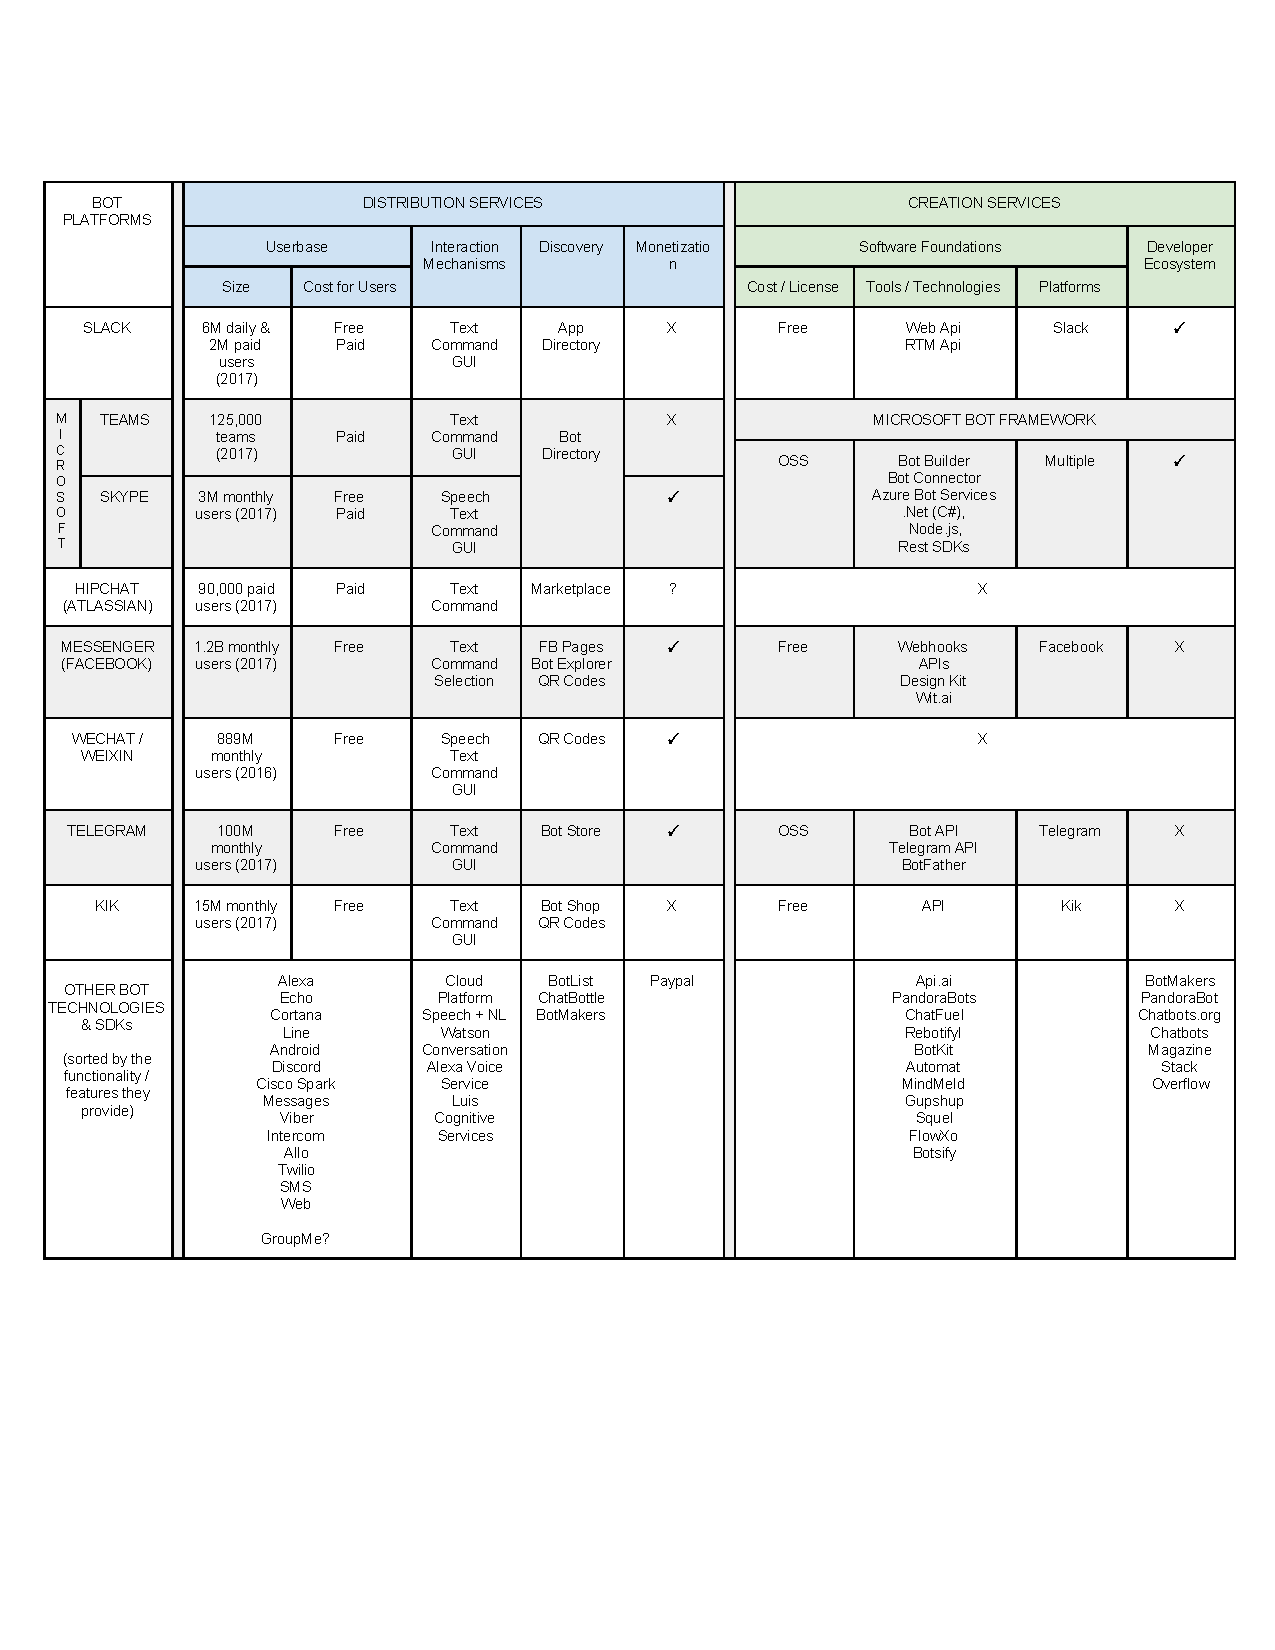
\includegraphics[width=\textwidth,height=400pt]{PlatformComparisonTable.pdf}
	  \caption{An overview of features for popular bot creation and distribution platforms.  The final entry in the table contains a collection of additional bot development technologies, sorted by category.}
	\end{figure*}

	Although simple bots can be built from scratch and self-hosted, many developers choose to leverage third-party frameworks to streamline the creation and distribution process. With the explosion of new tools in the bot development domain, we need to distinguish between the tools used to build bots (Creation Platforms) and the platforms where the bots dwell (Distribution Platforms).
%
% why no footnote for Microsoft?
	Large companies, such as Microsoft and Facebook\footref{Facebook}, offer a comprehensive set of tools to support both the creation and distribution of bots. Other companies, provide specialized solutions for specific aspects of bot creation and distribution. 

	\subsection{Distribution Platforms}
	Distribution platforms are online ecosystems where bots reside and function. These platforms dictate where and how the bots are accessed by end users. Many of these platforms are messaging or social networking platforms (e.g., Messenger, Skype, WeChat).  But other platforms are domain specific channels (e.g., Slack\footref{Slack}, Teams\footref{Teams}, and Hipchat\footref{Hipchat}) aimed towards software developers.  
	% are there domain specific for other domains? 
	These platforms support human(s)-bot, bot-bot, or even system-bot interactions.  

	Selecting the right distribution platform can lead to many benefits for developers.
	Some provide access to an existing user base\footnote{https://medium.com/mobile-lifestyle/messenger-vs-skype-vs-slack-vs-telegram-how-to-spot-the-winners-adc34b4ca066\label{How_to_spot_the_winners}}.
	Launching a bot on an existing platform gives developers a head start in overcoming the cold-start user problem that many new applications face. 
	% Selecting the wrong user base can be equally detrimental. 
	Developers should not only consider the size of the existing user base, but also the general user demographics as well as the costs for a user to access the platform.   
	Many distribution platforms define and standardize how users can interact with bots.  Such platforms have built-in support for commands, natural language, speech, and even rich UI controls.  The method of interacting with the bots, strongly influences the users' experience with the created bots.
	
	Many distribution platforms offer discovery mechanisms\footref{How_to_spot_the_winners} with different ways for users to discover and try out new bots. Similar to Apple's App-Store\footnote{http://www.apple.com/ca/ios/app-store/}, some platforms offer virtual ``bot stores'' where users browse for bots. Third-party sites (e.g., BotList\footnote{https://botlist.co/}, Chatbottle\footnote{https://chatbottle.co/}) also provide online catalogs of bots for many popular distribution platforms. These ``bot stores'' and catalogs are an easy way for bot developers to promote and market their bots. 
	Mature distribution channels also have monetization features\footref{How_to_spot_the_winners}, with a mechanism for the bots to safely collect payments from users, which can be particularly usefully when developing transactional style bots.

	A summary of popular distribution platforms and their associated technologies is included in Figure 1.  This is not a comprehensive list of all possible platforms, but rather a sample of popular technologies that developers can leverage.

	\subsection{Creation Platforms}

	The creation platforms support the design and development of bots. They provide a variety of software foundations, frameworks, toolkits, APIs, as well as other advanced features such as natural language processing, search, image processing, etc. These bot creation services may be platform specific or produce bots that can be deployed across multiple distribution platforms such as Microsoft Bot Framework\footref{https://dev.botframework.com/}, BotKit\footnote{https://www.botkit.ai/}, PandoraBots\footnote{https://www.pandorabots.com/}. 
	
	The services these creation platforms provide range from documentation and code templates, to no-code-required bot building interfaces such as ChatFuel\footnote{https://chatfuel.com/}. 
	Many of the popular bot creation platforms also belong to vibrant developer ecosystems. Developers can plug into these online communities for developer expertise in the form of tutorials, articles, discussions, and support.  Other general bot development communities, such as the BotMaker's Slack group\footnote{https://botmakers.org/} and the Chatbot New Community\footnote{http://news.chatbotsmagazine.com/}, are a hotbed for discussions on a variety of bot-related topics.

	A summary of popular creation platforms and their associated technologies is also included in Figure 1.


%	\section{Bots for Thought} or...
%	\section{A Few Thoughts on Bots} or...
 \section{Thoughts on Bots}
	
% [Peggy]

	These days, bots are rapidly becoming pervasive.  End users experience them in cars, in the home, in entertainment devices and at work, and as we discussed in the sidebar they play a significant and sophisticated role in many software development projects.  
	We need to learn from these early adoption experiences so that we find out what works well, but also what may go wrong when they are used.  We conclude this column with some advice we have gleaned about how best to use bots (or not).   
	But we encourage developers to form their own opinions as they observe how bots are used. 
	
	
	\subsection{To bot or not: amplify don't replace collaboration}
		Bots are frequently used in group or collaborative settings and 
		today it has become easy to automate many of the tasks that would normally require human interaction. But removing collaboration opportunities can have detrimental effects on creativity and productivity. 
		Rather than replacing collaboration, bots may be used to reduce friction in communication or task coordination. For example, bots may provide transparency  on task progress, make team goals more visible, link experts in a team with novices, as well as build team trust and cooperation \cite{lebeuf2017software}.
		However, bot overuse or poor design may lead to information overload and to too many interruptions---something bot designers need to be aware of and to watch out for.  

	\subsection{Bot or human? The user should always know what to expect}

	Unlike traditional Turing bots proposed back in the 1950s, bot developers should make it clear to the user that they are not speaking with another human but they are interacting with a bot. 
	Similarly, if a bot passes control to a human (when for example the bot cannot understand a command or answer a question), the user should be aware of this and the handover should be handled gracefully and transparently. This insures the user doesn't lose trust with the system supported by the bots and the user understands why control is being passed to a human. 
	It is also important that the purpose of the bot (what it can and can't do) be evident and should match the user's expectations. 
	%Another issue arises when bots try to be everything to everyone at once; it's better to do one thing well than many things poorly. Since the bot paradigm is still relatively novel, many users are willing to overlook some shortcomings.  To minimize disappointment and user frustration, Facebook's bot best practices recommends clearly defining expectations with the bot's users. This includes how often the bot will be responding, what core functionality it supports, and when it is unable to complete a request.  When a bot does not understand, it should reiterate it's capabilities or direct users to it's help functionality.


	\subsection{Bot talk: How to talk to and be heard by bots}
	% Control the conversational flow}

	Ideally, a user's interaction with a bot should be smooth and frictionless. 
	This can be achieved if the designer carefully plans potential conversational flows, especially for bots that are conversationally based.  For example, bots need to repeat the users' commands so the user knows they are listening and they need to be able to detect dead ends in a conversation and prompt the user by giving hints on how to continue the interaction. Some bots may incorporate UI elements (as mentioned above) to reduce the number of user clicks required and to make the conversation more efficient. 
	Implementing global input checks for common navigational keywords (help, back, cancel, start over, exit) can help avoid the creation of ``stubborn'' or ``clueless'' bots\footnote{https://docs.microsoft.com/en-us/bot-framework/bot-design-principles}.
	While tools like BotMock\footnote{https://botmock.com/} can be used prototype the user's ``journey through your bot''. 
%
%They should be guided through their interactions, through carefully planned out conversational flows. Avoiding using stand alone questions or dead end statements, and instead provide hints into the bots functionality with syntax hints and UI elements (buttons, menus, lists) where appropriate. 
%	A bot is more likely to be successful if it solves a user's ``problem better/easier/faster than any of the alternative experiences''\footnote{https://docs.microsoft.com/en-us/bot-framework/bot-design-principles}.  Clever use of rich UI elements, such as buttons and quick-replies, greatly reduce the number of clicks required per task.  Commands provide accelerators for speeding up an expert or mission driven user's navigation.
%
	Finally, many platforms have specific guidelines one can follow, e.g., Facebook recommends their bots follow a set of simple conversational guidelines\footnote{https://developers.facebook.com/docs/messenger-platform/introduction/design-best-practices}. 
	%Bots should use they active voice, in first or second person as appropriate.  Punctuation also plays a large role in the way the bot is perceived, so it can be leveraged to convey emotion but not at the expense of good grammar.  Lastly, proper spelling, capitalization, and sentence structure ensure that the meaning behind the message is not lost.


	\subsection{Bot personality matters more than looks} 
	As bots are predominantly textual based, how a bot uses language and even how it is named, influences the users' perception of its personality.  This may seem surprising given that users should know they are interacting with a mere program, but early research has shown that personality changes how users interact with them. 
	% A bot's choice of language helps define and build its personality.  
	Even if a bot can effectively accomplish a user's tasks, they won't adopt the bot if they find the bot boring. The choice of language should be casual, accessible, friendly, and fun.  Bots should expect users to test their abilities and respond accordingly.
	%like conversations in general, are more casual than many other company-user communication channels (e.g. websites, emails).  Bot's should aim to use friendly, accessible language and repeat inputs back to the user to they know it's listening. But developers should also feel free to have a bit of fun with users trying to test the bot (e.g. entering random inputs or repeating the same question). 
	But too much personality may not be a good thing.  According to Slack\footnote{https://api.slack.com/best-practices/}: ``A little goes a long way.''  Done right, bots can accentuate a company's brand and enhance culture.
	% We cannot say this enough.'' 
	% A bot's personality should accentuate their company's brand or fit seamlessly into their team's culture.  

\subsection{Bots should do no harm}

% 	Another challenge they may introduce includes privacy intrusion. 

Bots, like robots, should do no harm to users.  
Asimov's laws for robots~\cite{asimov1950evitable}, which include: 
	robots shall not harm humans; robots will obey orders; and robots will protect themselves; perhaps also apply to software bots.
	But perhaps these rules are too simple with the complexity and rapid growth of bots in our software ecosystems.  Simple mistakes could have devastating effects, and a user's privacy may be hard to protect.  
	We can expect to see a code of ethics in the near future for human-bot interaction, but in the meantime, developers should carefully consider how the bots may be misused either intentionally or unintentionally. Of course, many bots are already seen as malicious, and thus building trust with users may also pose a challenge. 
	 In the meantime, many of the platforms that support the creation and distribution of bots also provide developers with basic principles or best practices for bot design (Microsoft\footnote{https://docs.microsoft.com/en-us/bot-framework/}, Facebook\footnote{https://developers.facebook.com/docs/messenger-platform/design-resources}, Slack\footnote{https://api.slack.com/best-practices/}).
	 But developers wishing to use or create bots for their end users need to be careful which bots they bring to life. 
	

\section*{Sidebar}

% [Peggy]
% why bots in SE
Software developers are early adopters and proponents of bots as they recognize their potential to enhance developer and team productivity, as well as significantly improve software quality \cite{storey2016disrupting}. 
% why so much adoption in SE; and some not really bots
The adoption of bots in software development has been eased by the fact that developers engage in communication and source code repository hubs, such as Slack\footref{Slack}, Microsoft Teams\footref{Teams}, Atlassian's Hipchat\footref{Hipchat} and GitHub\footnote{http://github.com}.  Slack, Team and Hipchat provide a number of integrations with other services, with many of these integrations being referred to as bots (although many of these integrations are more like a scripting language command line interface than a chatbot). \cl{this bit is a tad repetitive. Maybe we could mention the benefits like team visibility, ease of access for ``non-technical'' team members, etc?}
Furthermore, developers feel very much at ease at using the bot frameworks that are available in these platforms to create bots to address friction points they experience in their own development projects. 
 
We see bots fulfilling a number of specific development tasks. For example, bots provide support to developers by:
%\begin{itemize}
%\item 
automatically committing code after testing (Jenkins CI\footnote{https://plugins.jenkins.io/}); 
automatically creating bugs when a test fails (BugBot\footnote{https://smallwins.today/bugbot}); 
automatically merging pull requests after a code review (Travis\footnote{https://docs.travis-ci.com/user/notifications/}); 
automatically opening issues when a code quality concern is detected (Freud\footnote{https://www.slideshare.net/svenpeters/rise-of-the-machines-automate-your-development-54456075/56-Freud\_Botfor\_Pull\_Requests\label{Atlassian}});
automatically testing for user interface changes when a code change is submitted (CompareBot\footref{Atlassian}); 
helping teams manage complex complex builds and supporting deployment from within the chat environment (as Hubot\footnote{https://hubot.github.com/} does); 
centralizing service and performance monitoring (PagerDuty\footnote{https://www.pagerduty.com/integrations/}); 
and interacting with end users (at scale) to answer frequently asked questions and to analyze user feedback (ZenDesk's AnswerBot\footnote{https://www.zendesk.com/answer-bot/}).
%\end{itemize}

Bots are also making their way into the developer's IDE. For example, SlackOverflow\footref{StackOverflow} is a new bot that integrates StackOverflow into Visual Studio.  This bot leverages Microsoft's AI platform to help find the best information from StackOverflow to meet a developer's needs based on their development context. 
Developers can expect to see more and more bots being introduced into the tools and platforms they use for development related activities.  \cl{we have seen similar integrations (code reviews, github, etc) in IDEs, its interesting that they are now taking a ``bot'' or ``chat'' style roll}

% \noindent
% \subsection*{Reference} 
% \begin{enumerate}
% \item Margaret-Anne Storey and Alexey Zagalsky. 2016. Disrupting developer productivity one bot at a time. In Proceedings of the 2016 24th ACM SIGSOFT International Symposium on Foundations of Software Engineering (FSE 2016). ACM, New York, NY, USA, 928-931.	
% \end{enumerate}



%ACKNOWLEDGMENTS are optional
% Acknowledgements
%\input{Acknowledgements.tex}



%
% The following two commands are all you need in the
% initial runs of your .tex file to
% produce the bibliography for the citations in your paper.
\bibliographystyle{IEEEtran}
\bibliography{bot_paper} % sigproc.bib is the name of the Bibliography in this case

%\input{bios.tex}

\listoftodos
% You must have a proper ".bib" file
%  and remember to run:
% latex bibtex latex latex
% to resolve all references
%
% ACM needs 'a single self-contained file'!
%
%\balancecolumns % GM June 2007
% That's all folks!
\end{document}
